% Please add the following required packages to your document preamble:
% \usepackage{multirow}
% \usepackage[table,xcdraw]{xcolor}
% If you use beamer only pass "xcolor=table" option, i.e. \documentclass[xcolor=table]{beamer}
\begin{table}[H]
\caption{Comparison of the different bearing options available}
\label{tab:bearingsComp}
\centering
\begin{tabular}{|m{2.5cm} |l|m{9cm}|}
\hline
\cellcolor[HTML]{\CellColor}\textbf{Type}                    & \cellcolor[HTML]{\CellColor}\textbf{Cost} & \cellcolor[HTML]{\CellColor}\textbf{Additional} \\ \hline
\textbf{Pillow bearing}          &                                       &                                             \\
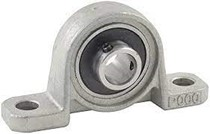
\includegraphics[width=\linewidth]{images/part9/bearing1.jpg}                              & \multirow{-2}{*}{£9.29}               & \multirow{-2}{\linewidth}{Bearing insert aligns with grub screw. Cost effective and light. Comes with clearance holes to increase modularity.}                    \\ \hline
\textbf{Deep grove ball bearing} &                                       &                                             \\
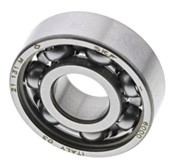
\includegraphics[width=\linewidth]{images/part9/bearing2.jpg}                               & \multirow{-2}{*}{£2.39}               & \multirow{-2}{\linewidth}{Would need welding to a section of the main structure. Cost effective and light.}                     \\ \hline
\textbf{Bolt oval housing}       &                                       &                                             \\
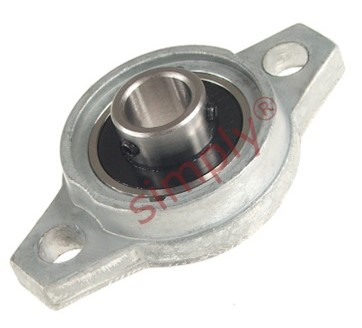
\includegraphics[width=\linewidth]{images/part9/bearing3.jpg}                              & \multirow{-2}{*}{£11.99}              & \multirow{-2}{\linewidth}{Bearing has two grub screws. Clearance holes would allow for modularity in the design. }                     \\ \hline
\end{tabular}
\end{table}